\documentclass[tikz,border=2pt]{standalone}

\usepackage{amsmath}
\usepackage{graphicx}
\usepackage{tikz}
\usetikzlibrary{arrows.meta, positioning, fit, backgrounds}

\begin{document}
\begin{tikzpicture}[
    font=\sffamily\small,
    >=Stealth,
    block/.style={draw, rounded corners=3pt, fill=white, align=center,
                  inner sep=5pt, minimum width=2.6cm, minimum height=0.85cm},
    eqbox/.style={draw, rounded corners=4pt, fill=blue!8, align=center,
                  inner sep=6pt},
    zbar/.style={draw, fill=gray!15, align=center, font=\sffamily\bfseries,
                 minimum width=2.6cm, minimum height=0.65cm},
    circnode/.style={draw, circle, fill=orange!15, font=\sffamily\small,
                     minimum size=0.8cm, inner sep=1pt, align=center},
    arrow/.style={->, thick},
]

% -- BACKBONE (encoder, left) ------------------------------------------------
% 3.2 cm wide x 4.2 cm tall
\node[draw, rounded corners=4pt, fill=white, align=center,
      minimum width=3.2cm, minimum height=4.2cm] (backbone) at (1.6, 4.2)
    {Backbone\\encoder $f$};

\node[align=center] at (1.6, 9.1) {Coordinates $(x,y)$};
\node[inner sep=0pt] (inp_img) at (1.6, 7.9)
    {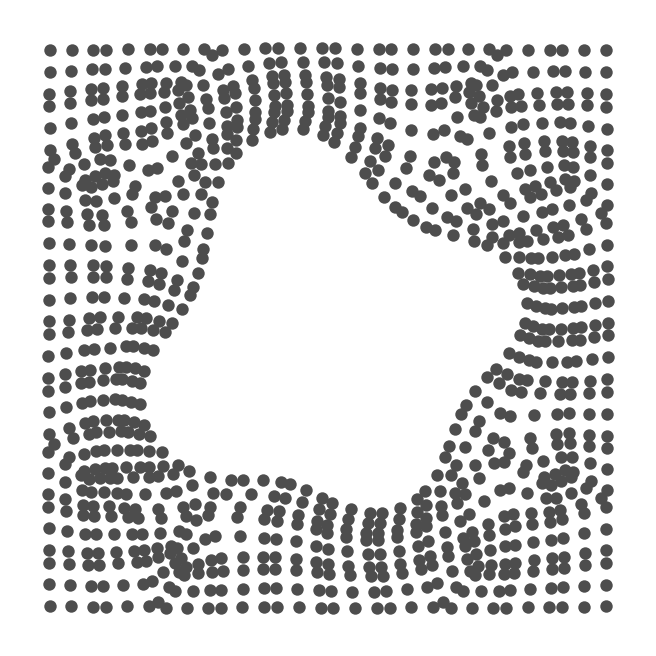
\includegraphics[width=2.2cm]{../../figures/elasticity/elasticity_diagram_input.png}};
\draw[arrow] (inp_img.south) -- (backbone.north);

% -- z BAR (small, bottom centre) -------------------------------------------
% x=4.0 is between backbone right edge (3.2) and constraint left edge (4.8)
% width=2.6 cm -> west at x=2.7, east at x=5.3
\node[zbar] (z) at (4.0, 1.1) {$z+(x,y)$};

% backbone -> z.west : down then left  (|- vertical first, then horizontal)
\draw[arrow] (backbone.south) |- (z.west);

% -- CONSTRAINT MODULE (dashed box, wider to fit math block) -----------------
\draw[dashed, thick, rounded corners=7pt, gray!65]
    (4.3, 2.1) rectangle (8.5, 6.3);
% \node[font=\footnotesize\sffamily\itshape, text=gray!55]
%     at (6.4, 6.65) {Constraint Module};

% --- MLP (bottom of constraint box) ---
\node[block, fill=gray!8] (mlp) at (6.4, 2.8) {MLP $\phi$};

% z.east -> MLP : right then up  (-| horizontal first, then vertical)
\draw[arrow] (z.east) -| (mlp.south);

% latent hooks: intermediate encoder features tapped straight into the MLP
\draw[arrow] (backbone.east|-mlp.west) -- (mlp.west)
    node[midway, above, font=\scriptsize] {latent hooks};

% --- Two circles: m and d (smaller, vertical arrows) ---
% placed at x = 6.4 +/- 0.9 so arrows from mlp and into const are vertical
\node[circnode] (m) at (5.5, 4.15) {$m$};
\node[circnode] (d) at (7.3, 4.15) {$d$};

\draw[arrow] ([xshift=-0.9cm]mlp.north) -- (m.south);
\draw[arrow] ([xshift=+0.9cm]mlp.north) -- (d.south);

% --- Constitutive law box: log-stretches -> principal stress -> von Mises ---
\node[eqbox] (const) at (6.4, 5.4) {
    $\lambda_i\;\to\; \boldsymbol{\sigma}(\lambda_i) \;\to\; \sigma_{\mathrm{VM}}$
};

\draw[arrow] (m.north) -- ([xshift=-0.9cm]const.south);
\draw[arrow] (d.north) -- ([xshift=+0.9cm]const.south);

% -- OUTPUT (above constraint box) ------------------------------------------
\node[inner sep=0pt] (out_img) at (6.4, 7.9)
    {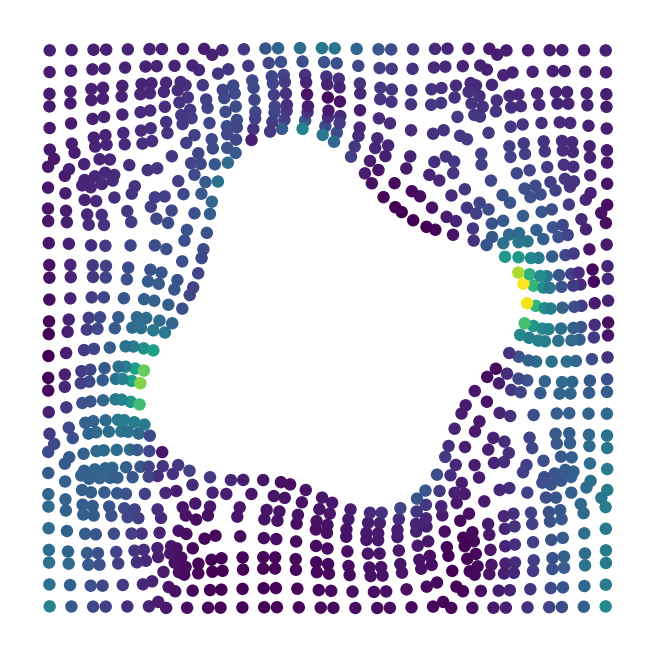
\includegraphics[width=2.2cm]{../../figures/elasticity/elasticity_diagram_output.png}};
\node[align=center] at (6.4, 9.1) {$\hat{\sigma}_{\mathrm{VM}}$};
\draw[arrow] (const.north) -- (out_img.south);

\end{tikzpicture}
\end{document}
